\documentclass{report}

    \usepackage{titlesec}
    \usepackage{listings}
    \usepackage{xcolor}
    \usepackage{titlesec}
    \usepackage[maxbibnames=99]{biblatex}
    \usepackage{tocloft}
    \usepackage{hyperref}
    \usepackage{enumerate}

    \renewcommand{\cftpartleader}{\cftdotfill{\cftdotsep}}
    \renewcommand{\cftchapleader}{\cftdotfill{\cftdotsep}}
    
    \titleformat{\chapter}{}{}{0em}{\bfseries\LARGE\ifnum\value{chapter}>0\relax\arabic{chapter}.~\fi}

    \lstset{ % General setup for the package
        belowcaptionskip=1\baselineskip,
        breaklines=true,
        frame=L,
        xleftmargin=\parindent,
        language=C++,
        showstringspaces=false,
        basicstyle=\footnotesize\ttfamily,
        morekeywords={PsSetCreateProcessNotifyRoutineEx2},
        keywordstyle=\color{blue},
        commentstyle=\itshape\color{purple!40!black},
        identifierstyle=\color{gray},
        stringstyle=\color{orange}
    }

    \hypersetup{
        colorlinks,
        citecolor=black,
        filecolor=black,
        linkcolor=black,
        urlcolor=black
    }
    
    \title{Behavior Analysis and Detection of Bashware}
    \author{
        Andrei Mermeze
        \\ email \href{mailto:andrei.mermeze@gmail.com}{andrei.mermeze@gmail.com}
        \\ [1cm]{\normalsize Advisor: Phd. Dragos Radu}
    }
    
    \date{}

    \addbibresource{bibliography.bib}

    \begin{document}
    \pagenumbering{Roman}
    \maketitle

    \tableofcontents

    \pagenumbering{arabic}

    \chapter{Introduction}
    With the release of Windows Subsystem for Linux (WSL) in the "Redstone 1" version of Windows 10, consisting of two new kernel-mode drivers,
    lxcore.sys and lxss.sys, which implement more than  200 linux system calls, a new service, LxssManager, and other user mode components,
    a new attack surface has been revealed, one that was not covered by monitoring tools untill recent, and doesn't seem to be covered by
    anti-virus vendors.

    WSL provides a way of executing native 64 bit Linux binaries, also known as ELF64 files, on Windows 10. Since WSL is not virtualization
    based, the Linux processes running in WSL can access the same resources as the Windows processes, while not being monitored by existent
    tools or anti-malware solutions.

    \section{Motivation}
        Seeing that currently no anti-virus vendor tried to tackle this issue and develop a security solution that could cover this new
        complex attack surface, I have decided to do more research about WSL and try to come up with a full stack security solution that covers
        this attack surface.
        
        Moreover, seeing a proof of concept of a privilege escalation exploit I had another reason to think that developing a security solution
        for WSL was imperative.

    \section{Objectives}
        The main objective is to provide a partial solution to this new security problem. It should defend a system from bashware,
        suspicious interaction between WSL processes and Windows processes and to provide system administrators with enough logs to properly
        respond to incidents, while not disrupting the user experience. The monitoring and detection system had to be self contained in
        a software development kit (SDK), in order to be easily integrable by any third party AV vendors.

    \section{Personal Contributions}
        My personal contributions towards monitoring and detecting malicious applications that leverage WSL are comprised of a few behavioral
        heuristic algorithms for detecting potentially malicious applications that target WSL, techniques for monitoring Linux applications
        and stopping potentially malicious processes.

        Another personal contribution would be the discovery of a local denial of service attack that leverages an access violation vulnerability
        in lxcore.sys.

        Moreover, I have integrated this SDK in an application in order to exemplify real world usage and integration of the designed
        system. 
        %Moreover, to exemplify the usage and integration of the designed system, I have integrated this SDK in an application
        
    \section{Thesis Outline}
        The thesis can be divided in four main parts. The first part consisting of chapter 2 will contain the current state of WSL and how it can
        be used to run malicious programs, how it can be used to bypass monitoring tools and anti-malware solutions and explain some exploits
        that target WSL.

        The second part, ranging from chapter 3 to chapter 7, presents the technologies and the reasons why they were used in order to
        develop the application as a whole, its architecture along with some implementation details and finally the testing process.

        The third part consists of chapter 7 and will be dedicated to describing the detection algorithms logic and what steps I followed in
        creating them, as well as some implementation details and limitations.

        Lastly, chapter 8 will show possible developement directions for this project, how the current monitoring solution can be improved and
        how it could be extended to achieve more in-depth monitoring and more accurate detection.
        
    \chapter{State of the art}
    \section{Windows Subsystem for Linux}
        \subsection{WSL Main Components}
            \begin{figure}[H]
                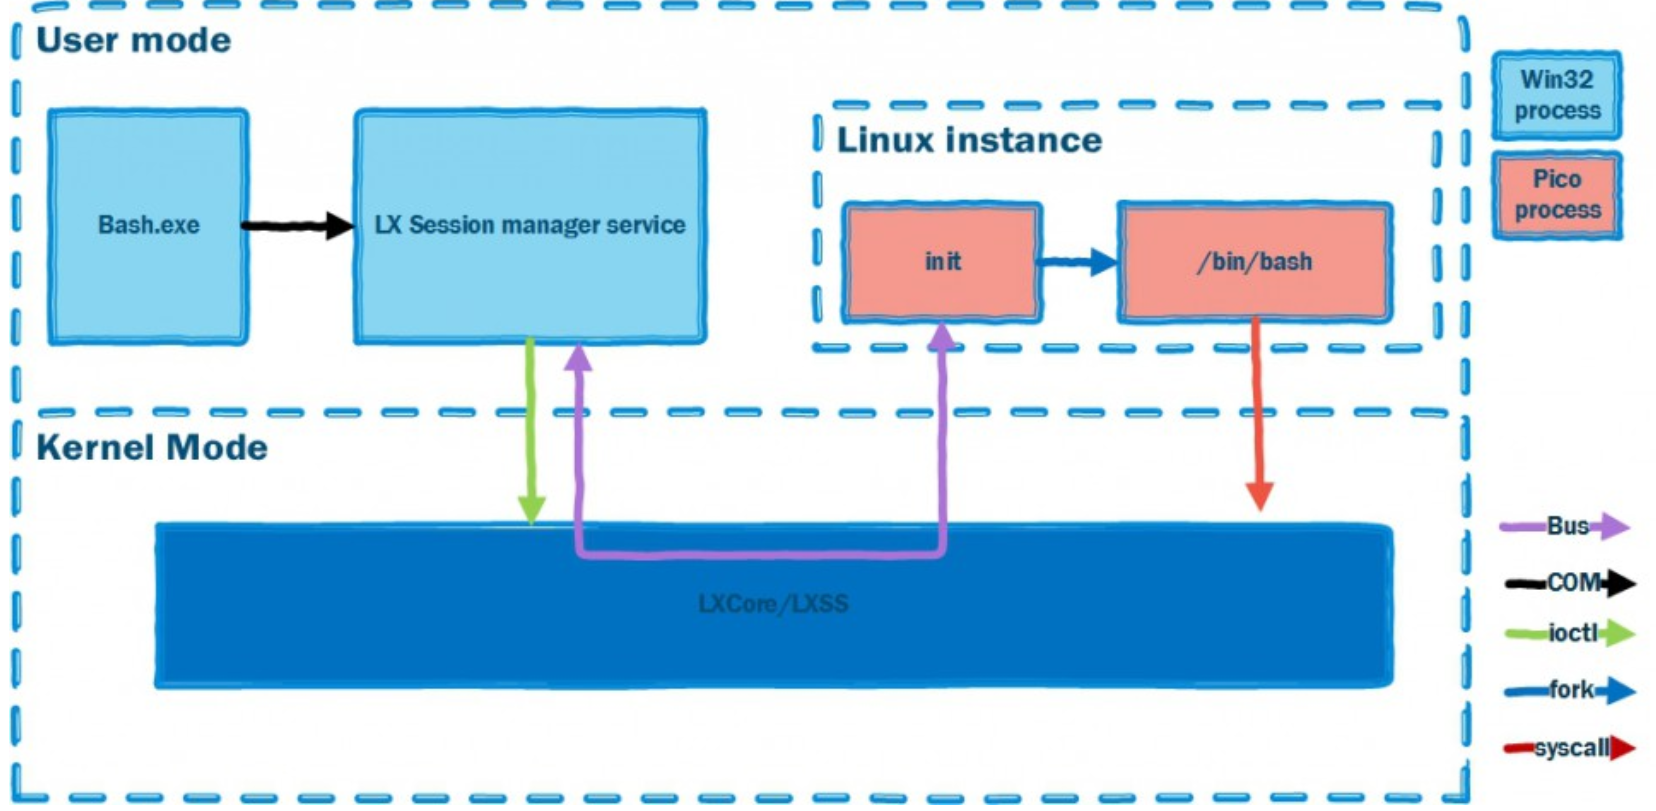
\includegraphics[width=\linewidth]{img/wsl_components.png}
                \caption{WSL Compoents \protect\cite{wslcomponents}}
                \label{fig:wsl_components}
            \end{figure}

        \subsection{WSL File System}
            \begin{figure}[H]
                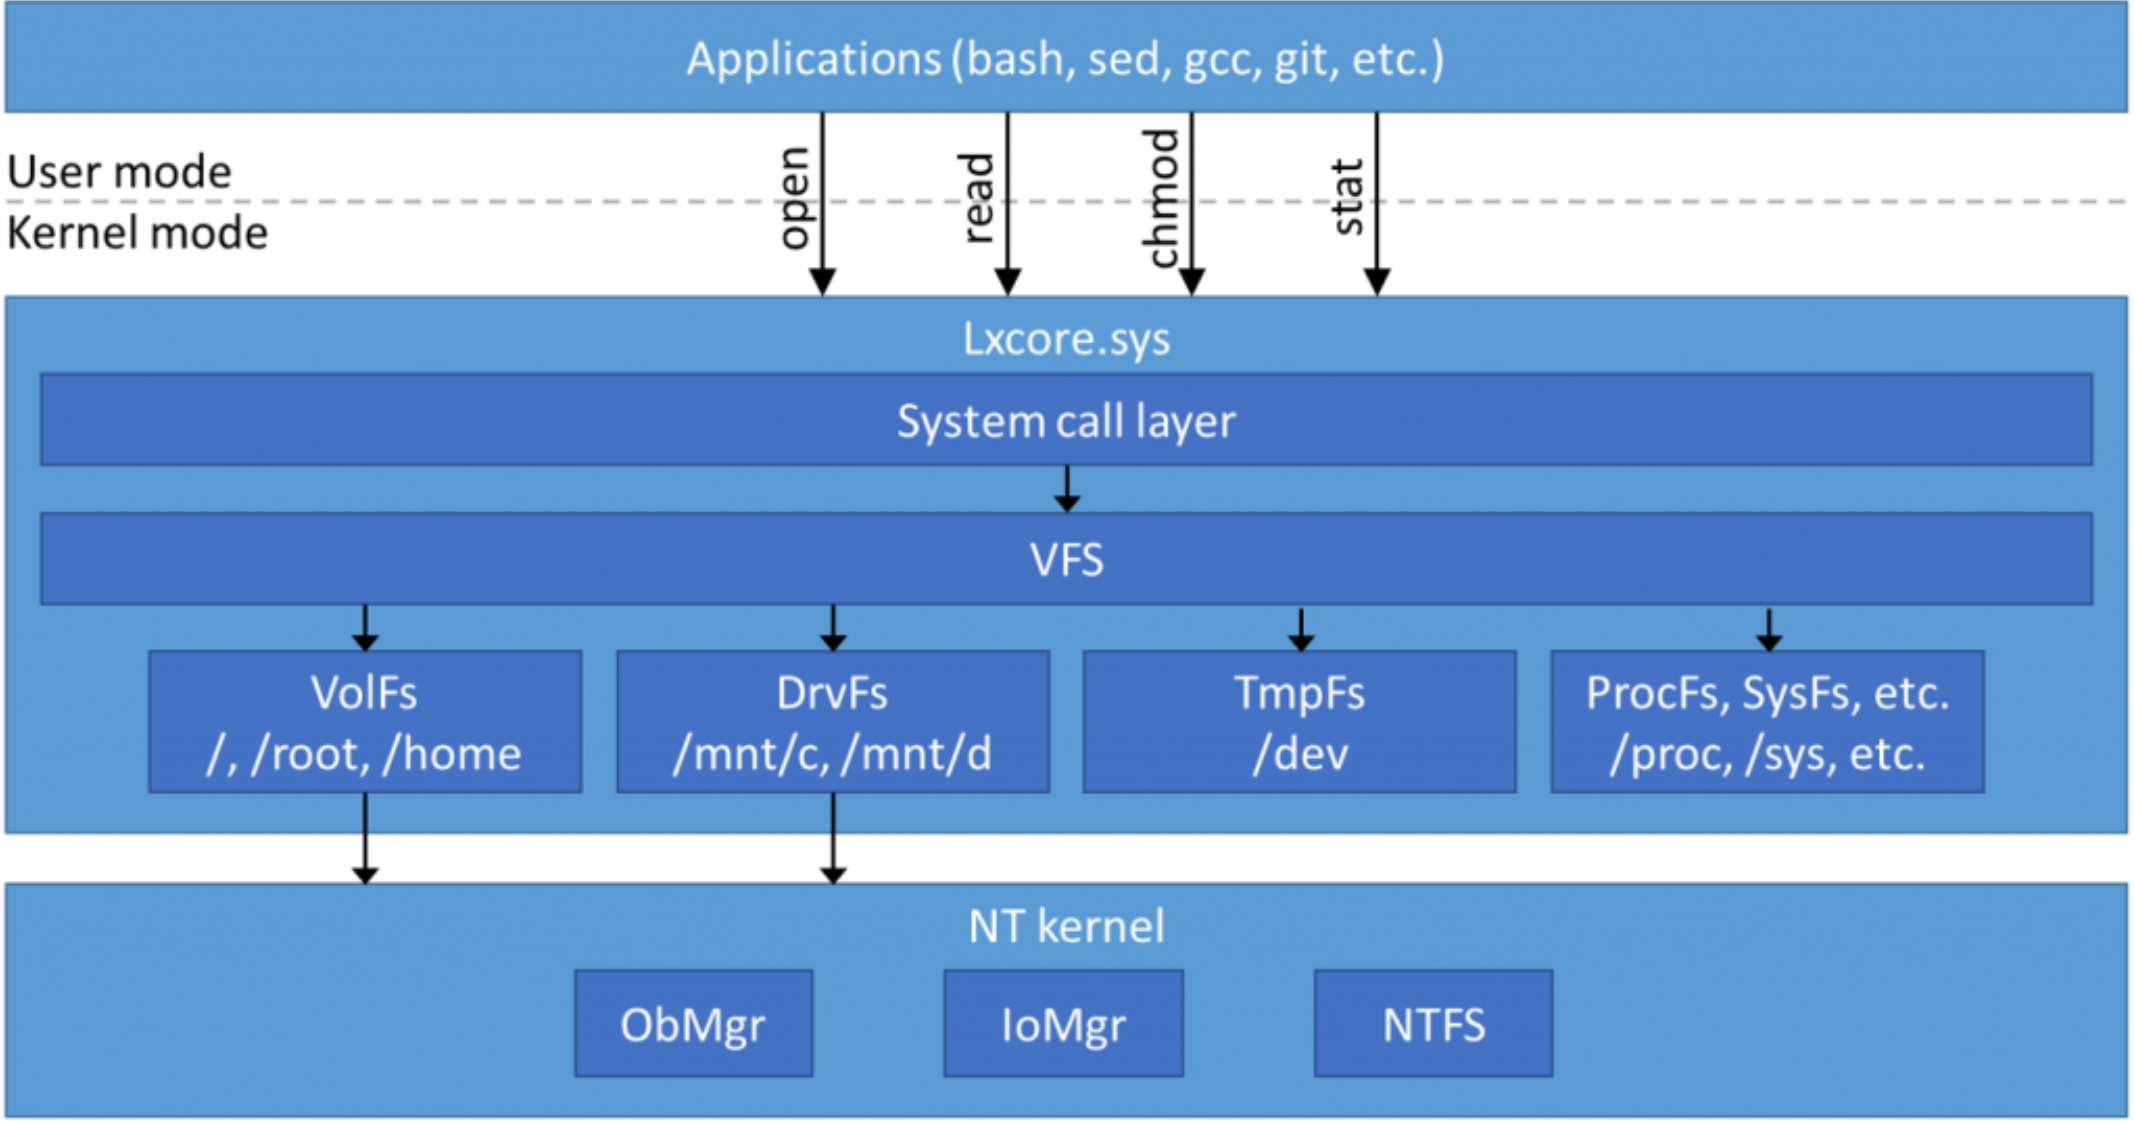
\includegraphics[width=\linewidth]{img/wsl_file_system.png}
                \caption{WSL File System \protect\cite{wslfilesystem}}
                \label{fig:wsl_file_system}
            \end{figure}

        
        \subsection{Security Issues}
        
        
    \section{Bashware and Exploits}
        \paragraph{}
        Bashware is a type of malware that leverages WSL in order to bypass monitoring tools and anti-virus products in order to do damage to the
        operating system.
        
        \subsection{execve exploit}
            \paragraph{}
            Discovered in February 2018 by Saar Amar, security researcher, is a privilege escalation exploit that leverages a vulnerability in
            lxcore, more exactly an integer overflow in LxpUtilReadUserStringSet. Starting from this vulnerability, the exploit proof of concept
            copies the system security descriptor over another process' security descriptor, elevating it at runtime.

        \subsection{File Infector}
            \paragraph{}
            A wsl file infector would essentially inject into windows executable files, altering the code in order to deliver some malicious
            code.
            
        \subsection{Local Denial of Service}
            \paragraph{}
            While experimenting with Event Tracing for Windows (ETW) I've found a way of consistently cause lxcore.sys to run into a Blue Scren
            of Death (BSOD), due to an access violation exception. This can be triggerd from a normal process with no admin rights. I will not
            go into more detail about this yet, as it would not respect the responsible disclore policy, since it wasn't yet fixed by Microsoft.
            Releasing information about how to trigger this local denial of service attack could cause exploitation in the wild.

    \section{Behavioral Detection}
        \paragraph{}
        
    \chapter{Used technologies}
    \section{File System Legacy Filter and Minifilter Drivers}
        \paragraph{}
        A Legacy Filter driver is a kernel-mode that could attach to a device's stack. In the context of file system filtering, these
        filter drivers could intercept file system I/O operations. Developing legacy filter drivers was quite troublesome and led to 
        many incompatibilities between filter drivers. This is one of the reasons for which minifilter drivers were added.
        
        \paragraph{}
        Minifilters have the same abilities as file system legacy filter drivers, but they are easier to develop and are overall safer. Their
        load order no longer depends on the attach order, but on a predefined value named altitude. Minifilters are managed by FltMgr, which is
        a legacy filter driver implemented by Microsoft.

        \paragraph{}
        I have used this technology for the core component of the developed application, which had to filter file system operations as well
        as process creation and termination. All of this information can't be reliably be acquired from a user mode application, so a minifilter
        driver was the only choice.

    \section{C++ in Kernel Drivers}
        \paragraph{}
        C++ has the advantage of being easy to use in developing coherent, object-oriented, robust and safe applications. However, msvc compiler
        does not, by default, support c++ in kernel drivers.

        \paragraph{}
        Firstly, in order to support global initializers, we need to define two sections, ".CRT\$XCA" and ".CRT\$XCZ". Between these two
        sections all pointers to global initializers are held.

        \paragraph{}
        Secondly, In order to support static object initialization, we need iterate through the list of global initializers and call each
        constructor in the DriverEntry function, and call the destructors during driver unload.

        \paragraph{}
        Thirdly, we need to define the global new and delete operators.

        \paragraph{}
        Lastly, we need to implement an the \textunderscore purecall() which will be called whenever a pure virtual function is called. Microsoft's implementation
        of this function causes the program to immediately terminate if there is no exception handler for it.

    \section{.NET Framework}
        \paragraph{}
        I have used .NET Framework for the integration project, both for the system service and the GUI application. The GUI was developed with
        the help of Windows Presentation Foundation (WPF), with the interface designed using Extensible Application Markup Language (XAML), and
        the communication between the service and GUI was done through Windows Communication foundation (WCF), more exactly, through the
        net.tcp protocol. WCF was particulary useful as it exposes an easy to use, RPC-like comomunication interface

    \section{C++/CLI}
        \paragraph{}
        The C++ modified Common Language Infrastracutre is a c++ based language specification developed by Microsoft. It offers the possibility
        to use both the unmanaged CRT heap (allocating and freeing objects) as well as the .NET managed heap, where objects are garbage collected
        and don't have to be freed by the programmer. This technology was helpful because it allows an easy linkage with a C or C++ DLL and
        provides a simple way of wrapping the dll's functions and classes in order to export them as .NET objects to .NET application, which,
        in this case, was a service.



    

    \chapter{Architecture}
    \section{High Level Overview}
        The system is composed of 2 main components
        \begin{itemize}
            \item wslmon - an SDK that contains the detection logic as well as communication logic between kernel-mode and user-mode
            \item wslam - the integrator
        \end{itemize}

        Below we can see a high level overview of the SDK and integrator components and how they can interract.
        
        \begin{figure}[H]
            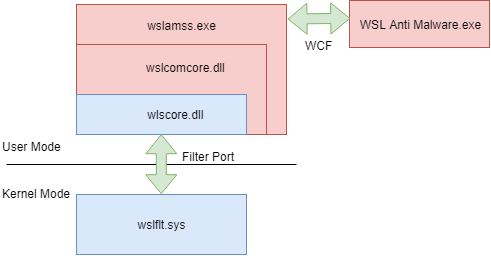
\includegraphics[width=360px, keepaspectratio]{img/high_level_overview_diagram.png}
            \caption{High Level Overview}
            \label{fig:high_level_overview_diagram}
        \end{figure}

        Blue colored components are part of the wslmon SDK, while the red colored components are the integrator components.
    
    \subsection{wslmon}
        Wslmon is an SDK that could be integrated by any OEM to include it in an existing security solution. Its
        architecture is meant to provide an easy way of integration in real anti-virus products, offer enough control of the system while
        encapsulating the monitoring and detection logic algorithms.

        The SDK consists of two components:
        \begin{itemize}
            \item wslflt.sys - a minifilter driver that encapsulates the monitoring, analysis and detection logic
            \item wslcore.dll - a shared library that provides an interface to communicate with the minifilter driver
        \end{itemize}

        \paragraph{wslflt.sys}
        is a C++ minifilter driver that contains the requirued sensors for monitoring process' activity. It's key components are the
        process filter, file filter, event dispatcher, the communication framework and the detection heuristics.

        \paragraph{wslcore.dll}
        is meant to ease the integration process of the SDK by third party anti-virus vendors. It offers an interface for controlling the driver
        state (enable/disable monitoring) as well as callback registration for several events (i.e detection).

    \subsection{wslam}
        Integrating the wslmon SDK, it consists of:
        
        \begin{itemize}
            \item wslcomcore.dll - C++/CLI DLL
            \item wslamss.exe - .NET Service
            \item WSL Anti-Malware.exe - WPF GUI Application
        \end{itemize}

        \paragraph{wslcomcore.dll} is built on top of C++/CLI to wrap wslcore.dll and export managed .NET classes
        for use in the .NET service. It's main purpose is to hide the filtering and detection logic and to provide an easy way to integrate
        the system in a complete security solution.

        \paragraph{wslamss.exe} contains the integration logic (ie. detection notifications, logging, etc) and serves as a communication
        endpoint, built using WCF framework, for the GUI application. It uses the previously mentioned dll to control the driver state, process
        driver's notifications as well as reqests sent from the GUI application. It is designed as a Windows Service application, therefore,
        making it easily convertible to an anti-malware protected process, once an Early Launch Anti-Malware (ELAM) driver is properly signed.

        \paragraph{WSL Anti-Malware.exe}
        is the GUI application that gives control to the user while also containing the user notification mechanism. It is designed as a system
        tray application in order to not distrupt the user experience, while the GUI itself is designed for usability.

    \section{SDK Architecture}
        The driver, which is responsilbe with monitoring of processes and detection of potentially malicious applicatoins, is comprised of
        two "sensors", the first being responsible of monitoring process creation and termination, called ProcessFilter, and the second being
        responsible of filtering file system I/O operations, called FileFilter.

        Most of the main components in the driver are implemented as singleton classes, and that is because of the inherent architecture of
        the minifilter APIs. For example, the callback for process notification has no context parameter, making it impossible to access
        any other component, except through singleton classes.

        This architecture is based on the single responsability principle, which states that a given method/class/component should have a
        single reason to change\cite{CleanCode}. Every component is self contained and self sufficient in order to be easily testable and
        maintainable.

        \subsection{Process Filter and Process Collector}
        The process filter is a stateful component, meaning that the filter can be enabled or disabled, and is responsible for registering
        the callback for process creation and termination notifications. It contains the logic for deciding whether a process should be
        monitored or not.

        It also contains a process collector, which is used as a database of active processes, internally represented by instaces of the Process
        class. A Process object holds the needed information for uniquely identifying the process throughout it's lifetime as well as other
        information useful for behavioral analysis, like the parent process, security token or command line.

        \subsection{File Filter}
        The file filter is also a stateful and singleton component. It's responsible for providing the IRP filtering callbacks and analyzing
        potentially malicious file system activity.

        Currently, the following operations are being monitored by the file filter:

        \begin{itemize}
            \item IRP\textunderscore MJ\textunderscore CREATE
            \item IRP\textunderscore MJ\textunderscore WRITE
        \end{itemize}

    \section{Integration Architecture}
    The SDK integration logic is encapsulated into a wslamss .NET Windows service application and is the juncture between the SDK and any 
    client application which would serve as a user interface.

    This architecture makes the integration project highly extensible, allowing the development of a central application that can monitor
    reported incidents and other events from multiple clients (systems with the anti-malware solution installed). For example, this could be
    useful for the network administrators or security reposibles in business environments, allowing for faster incident response.
    
    \paragraph{}
    The service has an external-facing WCF interface which is accessible trhough the net.tcp://localhost:8000. The metadata is available at
    net.tcp://localhost:8000/mex. The metadata exchange endpoint is done via SOAP messages that contain various information that describes
    the service, such as: available operations, parameter types, return types, callbacks that need to be implemented, etc. In other words,
    the metadata exchange endpoint exposes the WCF contract implemented by the service.

    \paragraph{}
    The settings, detection history and any other persistent data is saved in a local database that is managed with the help of SQLite
    database management system and .NET EntityFramework. This was the preferred choice as it doesn't require any special configuration on
    the user's machine. The only requirement is for the SQLite .NET assemblies to be present in the PATH environmental variable so they can
    be loaded by the service.

    Throughout the service application, we have two types of persistent data:
    \begin{itemize}
        \item detections history
        \item current settings
    \end{itemize}

    All this data is managed by the classes described below:

    \begin{figure}[H]
        \centering
        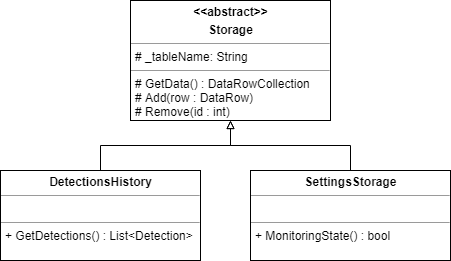
\includegraphics[width=300px, keepaspectratio]{img/storage_diagram.png}
        \caption{Data Persistence Diagram}
        \label{fig:storage_diagram}
    \end{figure}

    


        
    \chapter{Testing}
    \chapter{Testing}
    \paragraph{}
    Rigorous testing, especially in the context of kernel-mode modules and security solutions, is essential in order to provide a stable,
    usable and efficient product. Combining whitebox and blackbox techniques together with test driven developement paradigms throughout
    the development of a product is crucial in order to offer a high quality product.
    
    \section{Whitebox Testing}
        \paragraph{}
        In order to use the Test Driven Development paradigm, a whitebox unit testing framework was required. The unit test project contains
        mock definitions of kernel functions (e.g. ExAllocatePoolWithTag), and unit tests for each class. Mocking kernel functions helped in
        achieving high coverage of the driver code in a user-mode enviroment, thus saving development time. Moreover, these uni ttests can be
        easily configured to run at each solution build, making it a very reliable and easy to use continuous integration tool.
        
        \paragraph{}
        The other alternative was having another kernel-mode driver that would test the API exported by wslflt.sys. This is an unreliable
        and slow testing method because most bugs would cause a blue screen and can even corrupt the testing enviroment. Moreover, analysing
        kernel dumps in order to find bugs is a much slower process compared to analysing user-mode crashes or exceptions. Also, building a
        continuous integration system around this testing framework is a lot more complicated because it involves virtual machines,
        automatiically applying OS images and re-applying them in case a BSOD occurs.

        \paragraph{}
        In the context of the minifilter driver, whitebox testcases were implemented in order to verify that the Windows kernel APIs are
        correctly. These verifications include checks for handle leaks and correct error status handling. Moreover The driver's components
        (i.e. file filter, process collector) are tested individually to confirm that they work correctly. Also, generic framework classes like
        SharedPointer or LookasideObject are covered by unit tests as they are widely used throughout the project.
    
    \pagebreak

    \section{Blackbox testing}
        Blackbox testing, both manual and automated, is the main method of attesting a product's value, usefuleness and correctness regarding
        the users' needs. I have used blackbox techniques in order to verify both functional (i.e. detection) and non-functional requirements
        (i.e. stability, security, reliability).

        In order to identify memory or handle leaks, potential deadlocks, incorrect IRP handling, code integrity violation and other potential
        bugs, all blackbox tests are run with driver verifier enabled for wslft.sys. Using the driver verifier in the testing process helped
        in building a more robust and stable driver.

        Most blackbox testcases were implemented as bash scripts running in WSL, but some more complex testcases were also implemented
        using powershell.

    \section{Static Code Analysis}
        Static code analysis is a technique used to find potential bugs in a software without actually running it. Most code analysis tools use
        either the source code itself or some form of intermediate form of the code, (i.e. object code).

        SAL is a source code annotation language developed by Microsoft for C and C++. Its purpose is to clarify the intent behind the code,
        locking behavior or function parameters while also enabling static code analysis.

        Below is an example of SAL annotated function:

    \begin{Verbatim}[fontsize=\small, commandchars=\\\{\}]
\textcolor{magenta}{_Must_inspect_result_}
\textcolor{blue}{void} * memcpy(  
    \textcolor{magenta}{_Out_writes_bytes_all_}(count) \textcolor{blue}{void} *dest,   
    \textcolor{magenta}{_In_reads_bytes_}(count) \textcolor{blue}{const void} *src,   
    \textcolor{magenta}{_In_} \textcolor{blue}{size_t} count  
);  
    \end{Verbatim}

        \textunderscore Must\textunderscore inspect\textunderscore result\textunderscore
        - indicates that the return value of the function must be checked

        \textunderscore Out\textunderscore writes\textunderscore bytes\textunderscore all\textunderscore (count)
        - indicates an output parameter where we write exactly "count" bytes

        \textunderscore Out\textunderscore read\textunderscore bytes\textunderscore (count)
        - indicates an input parameter from which we read exactly "count" bytes

        \paragraph{}
        During code analysis, all these annotations are checked and any anomaly (i.e. writing to an \textunderscore In\textunderscore {} parameter) is
        reported as a compilataion warning.

    \section{WHQL Testing}
        In order to release a driver to the market, it needs to be digitally signed by microsoft, and the only way of receiving the signature, it
        must pass the WHQL test suite. In the case of wslflt.sys, that would be the Filter Driver Test Suite. These complex test suite
        contains extensive checks for reparse point handling, I/O stress conditions, transactional I/O, code integrity checks and much more for
        multiple file systems.

    \chapter{Performance impact analysis}
    \chapter{Possible improvements}
    This being a partial and basic solution to the problem, there are many improvements that can be made, for functional aspects like detection,
    and monitoring capabilities as well as for non-functinoal aspects, like performance, usability and overall robustness of the application.

    \section{Performance}
        There are multiple components that could be further optimized, for example, as of current implementation, the process collector is
        a doubly linked list, which is very inefficient for lookups (O(n) complexity). A more efficient implementation would be a resizable hash
        table using quadratic or lilnear probing. Another example of a component that needs optimization is the dictionary used to match paths
        for which we recheck the security token. A better implementation would use a compressed trie and aho corrasick algorithm for matching
        the path.

        Another performance improvement would be to not rematch the path for the same opened file each time we encounter it, but to cache
        the results in a minifilter define structure called "context", which can be attached to any filter manager object (i.e. file object, 
        volume, instance, etc.).

    \section{Detection}
        Currently, only privilege escalation is covered and, partially, file infectors. A very important type of malware that should be covered
        is ransomware. Ransomware is a type of malware that encrypts files and asks for a ransom, usually in the form of cryptocurency, in order
        to decrypt the user's files.

        \paragraph{}
        Moreover, detection could be improved by integrating next-gen anti-virus features, like AI based detection. Multiple solutions are
        possible and should be investigated, for example Markov Model and Markov Chains or Recurent Neural Networks. These could prove extremely
        efficient because most of the complexity is in the training of the model, while using the model in order to identify malicious actions
        would just follow a simple linear algorithm.

        \paragraph{}
        Finally, in order to more reliably and efficiently detect exploits in general, especially kernel exploits, memory introspection
        techniques could be implemented at hypervisor level. ) Hypervisor perform virtualization without a host operating system between them
        and physicalsystem hardware\cite{Bulazel}. The Xen hypervisor \cite{Barham} has been used in several surveyed analysis systems.
        
        For example, privilege escalation could by detecting by hooking memory access at process security tokens and making use of Extended
        Page Tables (EPT).
        
    \section{Reverting malicious actions}
        In case of behavioral detection, a process could do some malicious actions before being detected. For example, a ransomware may actually
        encrypt some files or parts of some files before being stopped by the anti-virus solution. In this case, it would be needed to store all
        permanent actions (i.e. file delete) and revert them when and if the process is detected.

    \section{Network Filtering}
        A network filter kernel-mode driver is required in order to monitor and report suspicious network activity inside WSL. For example, such
        a component could possibly detect reverse shell behavior.

    \section{User-Mode Hooking Framework}
        In order to obtain more granular monitoring capabilities, a function hooking framework is required. The ability of synchronously monitoring
        specific API usage opens up a range of possibilities, from exploit detection to syscall graph based detection heuristics.
        In order to load a shared library into any Linux pico process, an entry with the path to the library must be added into the ld.so.conf. Since
        any process with root privilleges (inside the linux system) can update the said config file, we must protect it from a kernel driver, so that
        we are sure that our shared library isn't removed. This can be done by filtering IRP\textunderscore MJ\textunderscore WRITE operations on that
        file and readding the entry if removed.
        
        When loaded in a linux process, the library hooks the functions we want to monitor (i.e. ptrace, open) and synchronously notifies a 
        service via local sockets about every hooked function call, informing the service about exploitation intent and failing the function call
        if needed.

        We consider this method unreliable against smarter bashware that actively checks and avoids hooked functions, and possibly completely useless
        starting with Windows RS5 if executable memory can't be allocated anymore.


    \titleformat{\chapter}{}{}{0em}{\bfseries\LARGE}
    \nocite{*}
    \emergencystretch=1em
    \printbibliography[heading=bibintoc, title={References}]

\end{document}